\chapter{Design \& Implementation}
\section{Vision Architecture}
    \begin{figure}[ht]
    \centering
            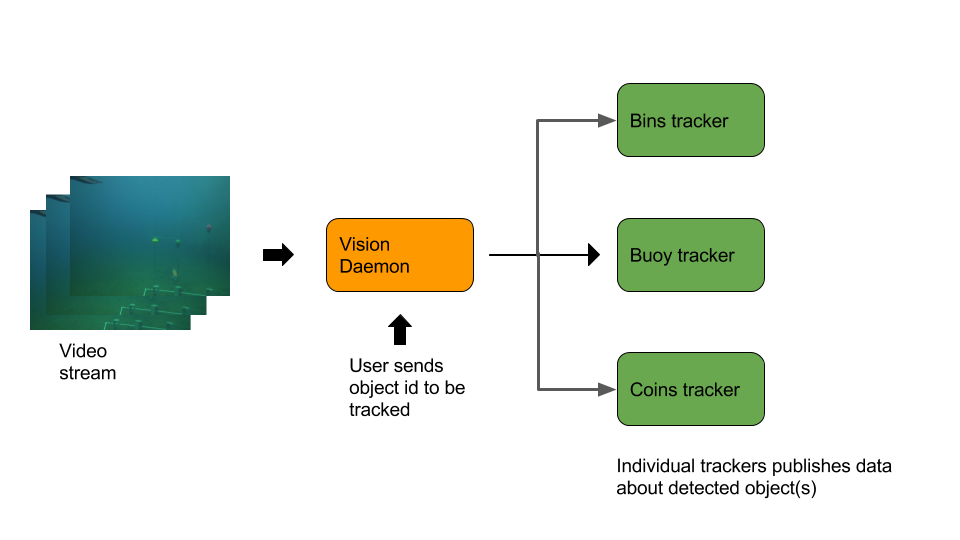
\includegraphics[width=0.8\textwidth, height=0.3\textheight]{overall_vision_architecture.png}
            \caption{BBAUV Vision Architecture}
            \label{fig:vision_architecture}
    \end{figure}
    
Our vision framework is implemented as a vision daemon running in the background when the AUV is launched. The vision framework is  integrated with ROS (Robotics Operating System) \cite{quigley2009ros}, an open source meta-operating systems used widely in robotics which provides message interface for inter-process communication (IPC). The vision daemon will initialized a new tracker upon request from the user (if the object is not currently being tracked). One advantage of this approach allows for parallel development of vision algorithms before competition which not speed up development but resulting in modular vision algorithms that are substitutable. 
\section{Methodology}
Individual object trackers are implemented using a tracking-by-detection approach where theese trackers had already been implemented and deployed in Robosub 2016. Below shows the vision pipeline of the baseline object tracker:
    \begin{figure}[ht]
    \centering
            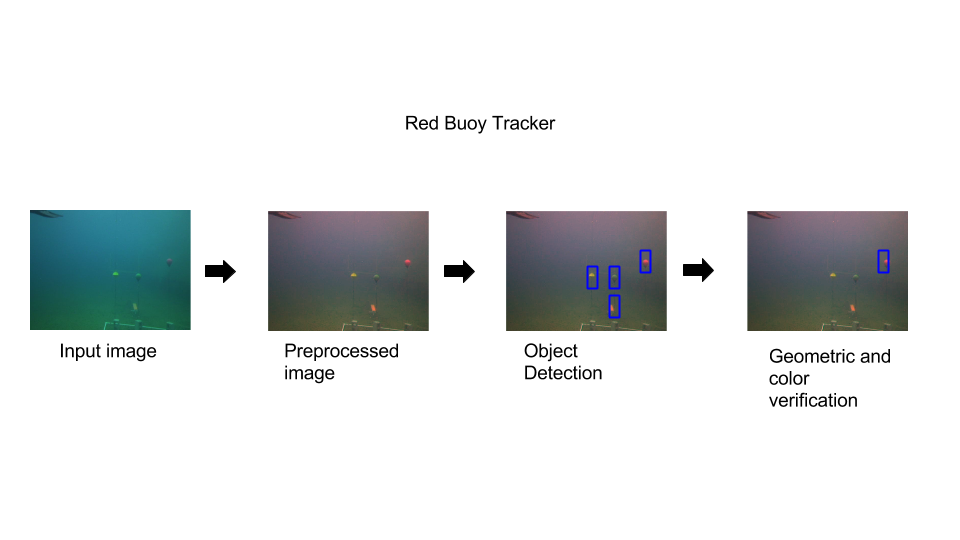
\includegraphics[width=0.8\textwidth, height=0.3\textheight]{object_tracking_pipeline.png}
            \caption{Object Tracking Pipeline}
            \label{fig:object_tracking_pipeline}
    \end{figure}
    
\subsection{Preprocessing} 
Input image first undergoes preprocessing before being processed by individual object detector. A design decision has been made to perform preprocessing on demand to a) reduce computation cost and b) customize preprocessing for different type of vision tasks. From past experiences, objects with distinct color from environment and bottom-facing objects can be detected without much preprocessing. Preprocessing can be separated into color constancy algorithms and underwater image enhancement algorithms. 

\subsubsection{Implemented Color Constancy Algorithms}
    \begin{figure}[h]
    \centering
            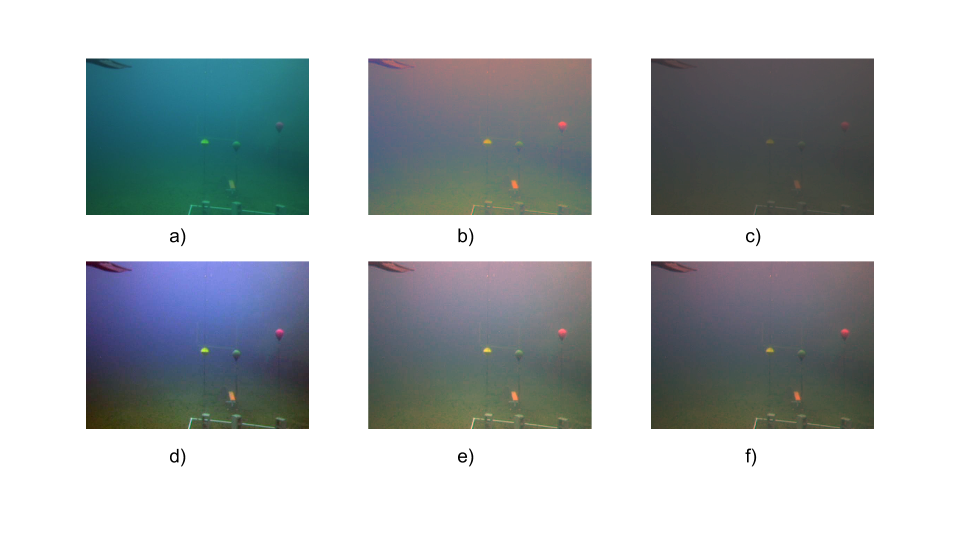
\includegraphics[width=0.8\textwidth, height=0.3\textheight]{color_constancy.png}
            \caption{Color constancy algorithms a) Original image b) Finlayson's comprehensive normalization c) Grey world d) Image Adaptive Contrast Enhancement (IACE) e) Non-iterative normalization f) Shade of Grey }
            \label{fig:color_constancy}
    \end{figure}
Various color constancy yields different results based on different underwater conditions. We can observe that some color constancy algorithms produce image with red hue which may affect performance of color-based object detectors. It must be known that gamma correction is performed after performing Grey-World algorithm to produce image with sufficient lighting. \outcite{Gijsenij2011} suggests that several approaches are combined to achieve optimal result. 

\subsubsection{Underwater Image Enhancement}
    \begin{enumerate}
        \item Gamma correction \\ To reduce effect of overexposure or underexposure because of camera settings. Sudden change in illumination because of cloud movement or position of the sun can be catastrophic.
        \item Homomorphic filter \\ To reduce flickering effect of bottom- facing tasks. This is implemented on the spatial domain \cite{nnolim2008homomorphic}
    \end{enumerate}
    
\section{Saliency Region Detection}
\begin{figure}[h]
    \centering
            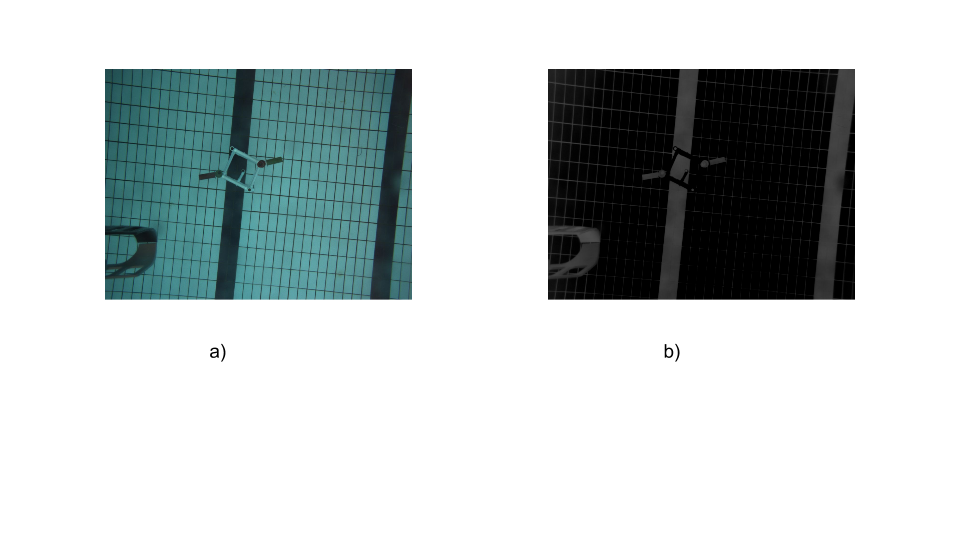
\includegraphics[width=0.8\textwidth, height=0.3\textheight]{saliency.png}
            \caption{Salient object detection of cylinders a) original image where color of cylinders severely degraded b) saliency map still mangages to capture the cylinders}
            \label{fig:saliency_detection}
    \end{figure}
The saliency detection approach of \cite{achanta2009frequency} is implemented to detect salient objects underwater as competition obstacles are often more salient than other features. Experiments have shown that images needed to be contrast enhanced and color corrected to achieve reliable detection. 
